\section{Ransac mit Maskierung \dcfirstauthorshort} 
\label{sec:maskenbau}

Der nun folgend beschriebene Ansatz zur Detektion der Fahrbahnlinien ist in der endgültigen Implementierung nicht zum Einsatz gekommen. Da wir uns jedoch lange Zeit damit beschäftigt und viele später weiter verwendete Grundfunktionen aufgebaut haben, wird die Vorgehensweise nun näher erläutert.

%Die Implementierung begann bereits vor Fertigstellung der Hardware. Zu jenem Zeitpunkt wurde deshalb der Bildausschnitt noch nicht so gewählt, wie in~\ref{fig:bildvorverarbeitung_entzerren} zu sehen, weshalb die Abbildungen~\ref{fig:fahrspurerkennung_ransac_binarisieren}, ~\ref{fig:fahrspurerkennung_ransac_masken} und~\ref{fig:fahrspurerkennung_ransac_ransac} einen anderen Teilbereich darstellen. Dies ändert indes nichts an dem Algorithmus selbst, sondern hängt lediglich von den gewählten Kamera- und Bildausschnitts-Parametern ab. 

Nachdem das Foto binarisiert wurde, stellen alle Pixel mit dem Wert \glqq 1\grqq{} im Idealfall potenzielle Linienpunkte dar. Diese müssen nun der richtigen Kategorie \glqq linke\grqq , \glqq mittlere\grqq{} oder \glqq rechte\grqq{} Linie zugeordnet werden, wenn sie nicht bereits mittels \gls{acr:ransac}-Algorithmus als Outlier (siehe Abschnitt \ref{ssec:grunglagen:ransac:ablauf}) markiert worden sind. Dazu legen wir je nach Zugehörigkeit eine entsprechende \gls{acr:roi} im Bild fest. Die Idee war, die Maske anhand unserer bereits eingetragenen Punkte in der Weltkarte und der Pose zum Zeitpunkt der Bildaufnahme zu kreieren, sodass nur die zur Linie zugehörigen Pixel an der erwarteten Stelle gesucht werden konnten. 
%Die Weltkarte ist ein Struktur-Feld, in dem unter anderem die Koordinaten der eingetragenen Linienpunkte gespeichert sind, jedoch nicht deren approximierte Funktion. 
Zur Gewinnung der entsprechenden \gls{acr:roi} werden eine bestimmte Anzahl der zuletzt eingetragenen Kartenpunkte gleichartiger Kategorie in das aktuelle Bild transformiert, welche folgend die Grundlage für eine Regression darstellen. Die daraus ermittelte Funktion bildet die Mitte der \gls{acr:roi}. Nach einer Dilatation des im Bildausschnitt liegenden Teils der Funktion um einen Parameterwert entsteht ein dickes Band aus Punkten, welche die \gls{acr:roi} beschreiben (siehe Abbildung~\ref{fig:fahrspurerkennung_ransac_masken}).

% entzerrtes und binarisiertes Beispielbild und Filterergebnisse für Mittellinie nebeneinander (4 Bilder)
\begin{figure}[H]
  \centering
  \subfloat[][]{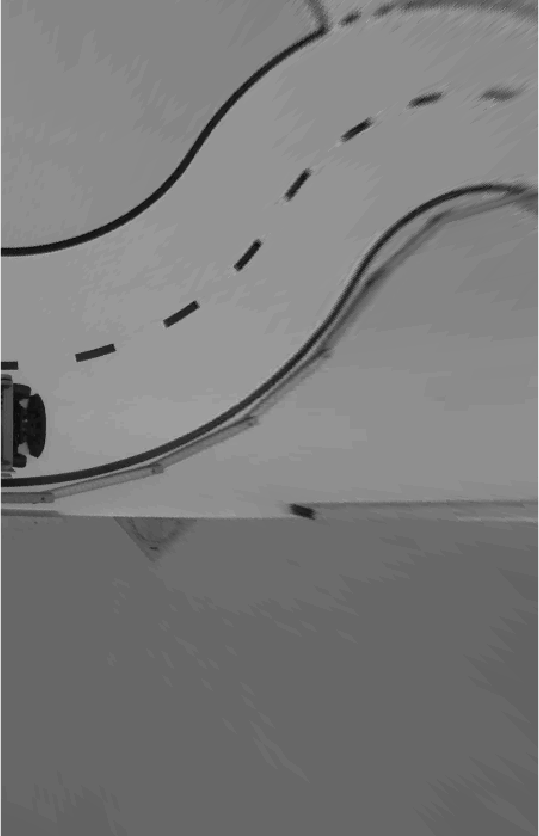
\includegraphics[width=0.4\textwidth]{fahrspurerkennung_ransac_imgUndist.png}}
  \qquad
  \subfloat[][]{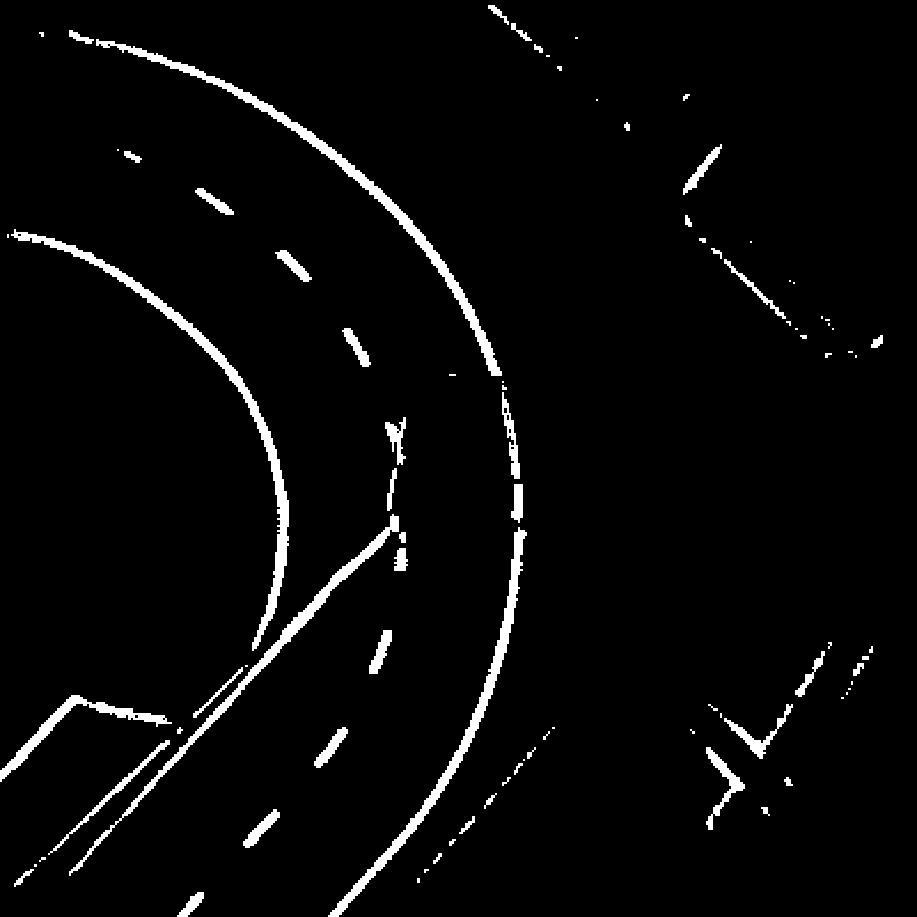
\includegraphics[width=0.4\textwidth]{fahrspurerkennung_ransac_imgBinarized.png}}
  \qquad
  \subfloat[][]{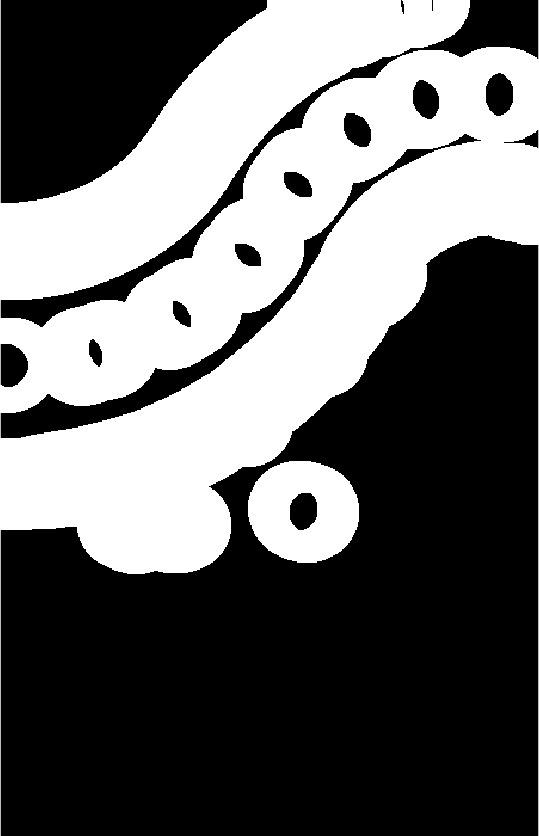
\includegraphics[width=0.4\textwidth]{fahrspurerkennung_ransac_imgMidFiltered.png}}
  \qquad
  \subfloat[][]{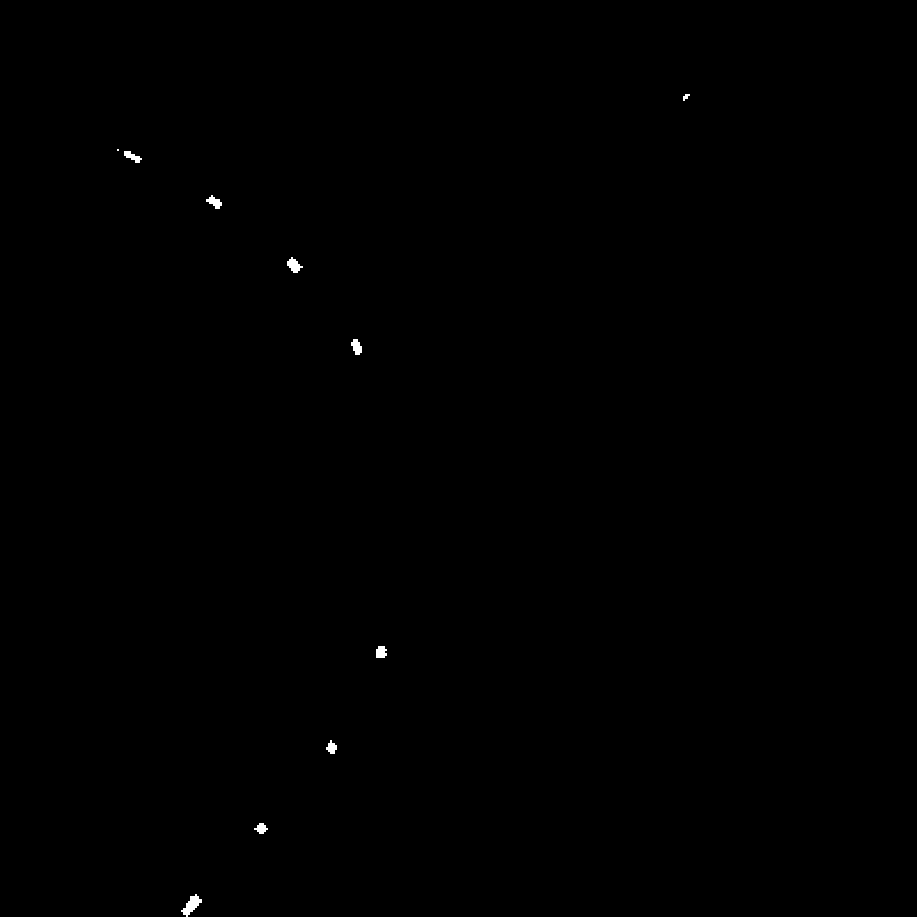
\includegraphics[width=0.4\textwidth]{fahrspurerkennung_ransac_imgBinarizedAndNotImgMidFiltered.png}}
  \caption{entzerrtes (a) und binarisiertes Bild (b) einer Testaufnahme auf der Strecke in alten Kameraeinstellungen; Filterergebnis des ''Ringfilters'' (c) und Durchschnitt dessen Negation mit dem binarisierten Bild (d)}
\label{fig:fahrspurerkennung_ransac_binarisieren}
\end{figure} 

% Textumflossenes Bild des ''Ringfilter''-Kerns
\begin{wrapfigure}{r}{0.5\textwidth}
 \centering
  
\includegraphics[width=0.3\textwidth]{fahrspurerkennung_ransac_midfilter.png}
  \caption{Der Kern des \\ \glqq Ringfilters\grqq}
\label{fig:fahrspurerkennung_ransac_midfilter}
\end{wrapfigure} 

\paragraph{Initialer Maskenbau} 
\label{par:maskenbau:initial}

Ein nicht zu vernachlässigendes Problem stellt allerdings noch die Initialisierung dar. Wie gewinnt man die Masken, wenn bisher keine Linienpunkte in die Karte eingetragen worden sind? Die einfachste und am Anfang auch implementierte Möglichkeit bietet die aus Parameterwerten vorgeschriebene Maske einer Gerade, in der Annahme, das Auto starte immer auf einem geraden Abschnitt. Da so die Robustheit aber schlecht gewährleistet ist, wurde dies schnell wieder verworfen und eine bessere Möglichkeit gefunden. Die gestrichelte Mittellinie besitzt im ganzen Bild Alleinstellungsmerkmale, die sich durch ein darauf angepasstes weiteres Faltungsfilter nutzen lassen. Den in Abbildung~\ref{fig:fahrspurerkennung_ransac_midfilter} gezeigten Filterkern haben wir \glqq Ringfilter\grqq{} genannt (Idee entnommen aus \autocite{drauschkeEchtzeitfaehigeStartpunktalgorithmenFuer2016}). Er ist aus einem Innen- und Außenkreis entworfen, sodass der Radius des inneren Kreises mindestens so groß wie die Länge eines Mittellinienstriches im Bild und der Außenkreisradius maximal so groß wie der kürzeste Abstand zwischen zwei Mittellinienstrichen ist. Was als Filterergebnis beispielhaft herauskommt, ist in (c) der Abbildung~\ref{fig:fahrspurerkennung_ransac_binarisieren} zu erkennen. Das Filter bewirkt, dass im Ergebnisbild genau dann ein Pixel mit \glqq 1\grqq{} beschrieben wird, wenn der Filterring um dieses Pixel mindestens einen Punkt im binarisierten Bild schneidet. Es entstehen abgegrenzte Bereiche mit einer \glqq 0\grqq{} als Filterantwort genau dann, wenn Mittellinienstriche innerhalb des \glqq Ringfilters\grqq{} liegen und kein weiteres Pixel auf dem Ring um diese Striche gefunden wird. Die Negation des Filterergebnisses als Maske auf das binarisierte Bild gelegt erzeugt eine Grafik, die allein Pixel aus Punktgruppen enthält, die eine festgelegte Maximallänge und einen Mindestabstand zu anderen Punkten besitzen. Darauf kann nun der \gls{acr:ransac}-Algorithmus angewendet werden. Dass hier der Einsatz von \gls{acr:ransac} sinnvoll und notwendig ist, erkennt man in (d) der Abbildung~\ref{fig:fahrspurerkennung_ransac_binarisieren} im unteren Teil des Bildes an der hellen Pixelgruppe, welche nicht zur mittleren Fahrbahnmarkierung gehört.

% Bilder der drei Masken über binarisiertem Bild incl. Fit für linke, mittlere und rechte Linie
\begin{figure}[H]
	\centering
	\subfloat[][]{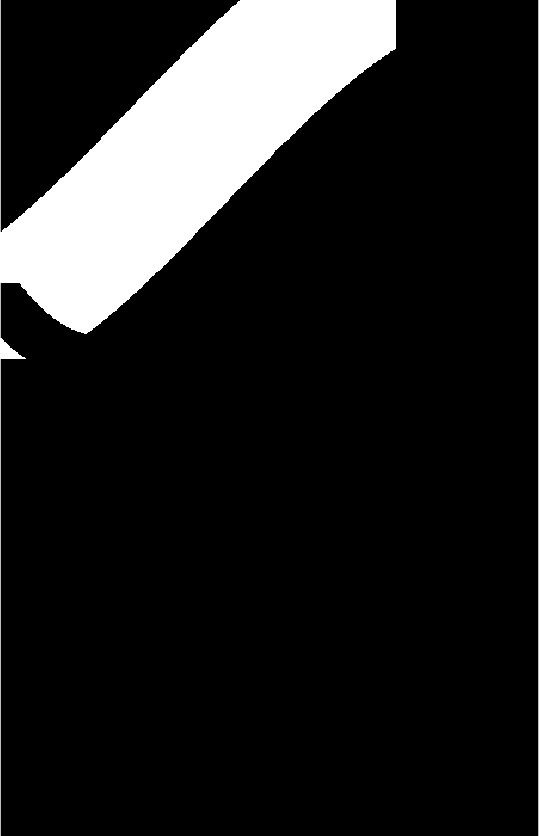
\includegraphics[width=0.3\textwidth]{fahrspurerkennung_ransac_imgMaskLeft.png}}
	\quad
	\subfloat[][]{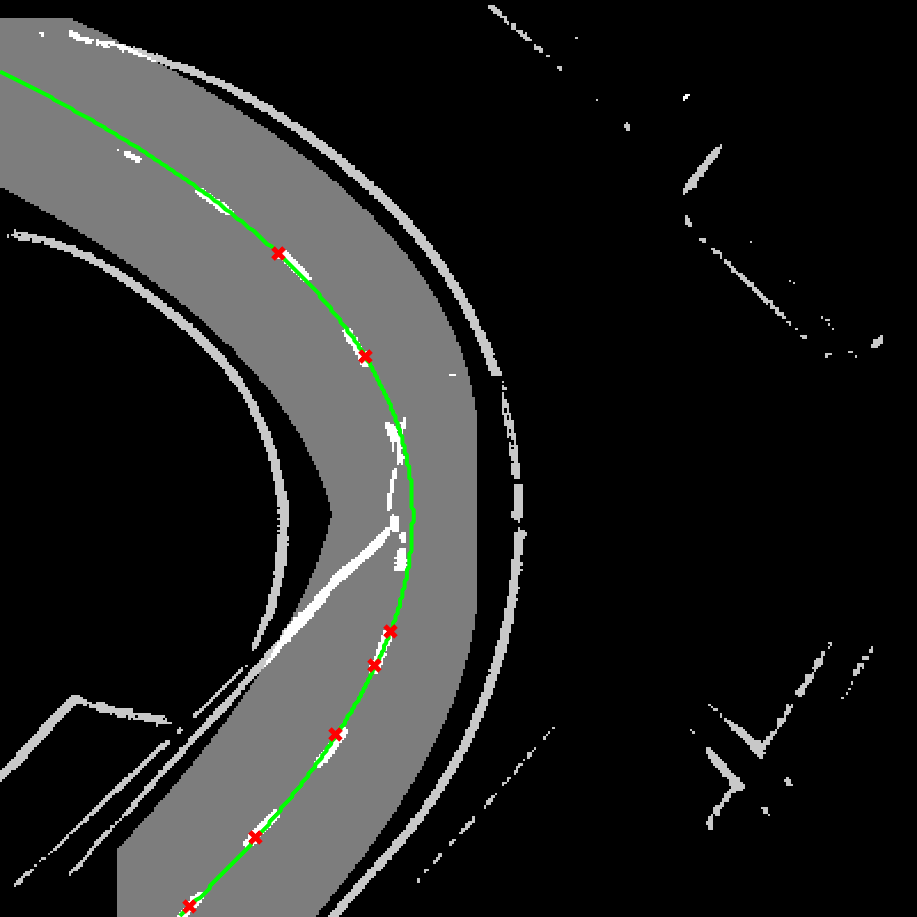
\includegraphics[width=0.3\textwidth]{fahrspurerkennung_ransac_imgMaskMiddle.png}}
	\quad
	\subfloat[][]{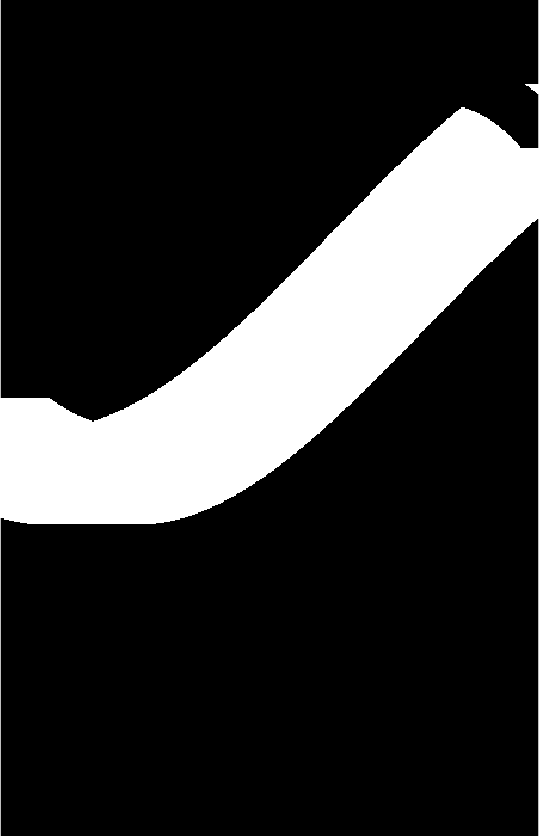
\includegraphics[width=0.3\textwidth]{fahrspurerkennung_ransac_imgMaskRight.png}}
	\caption{Masken zum Herausschneiden der linken (a), mittleren (b) und rechten (c) Fahrbahnmarkierung für die Anwendung des \gls{acr:ransac}-Algorithmus}
	\label{fig:fahrspurerkennung_ransac_masken}
\end{figure} 

Die zwei initialen Masken für die Randlinien werden anschließend aus der approximierten Funktion dritten Grades der Mittellinie gebildet. Dies geschieht aus der gerichteten Verschiebung diskreter Punkte der Approximation. Gleichung~\ref{eq:polynom3} sei eine mathematische Beschreibung der Funktion, die den Linienverlauf approximiert, dann ist Gleichung~\ref{eq:derr_polynom3} die Ableitung, welche den Anstieg an den Stellen \gls{x} beschreibt. Der Verschiebungsvektor \gls{lat:dv} steht dann senkrecht auf \( \mathrm{f} \).

\begin{eqnarray}
\mathrm{f}(\gls{x}) & = & a{\gls{x}}^3 + b{\gls{x}}^2 +c{\gls{x}} +d  \label{eq:polynom3} 	\\
\mathrm{f}’(\gls{x}) & = & 3a{\gls{x}}^2 + 2b\gls{x} +c \label{eq:derr_polynom3} 							\\
\gls{lat:dv} & = & \frac{1}{\sqrt{(-\mathrm{f}’(\gls{x}))^2 + 1}} \cdot
\begin{pmatrix}
-\mathrm{f}’(\gls{x}) 	\\
1 		\\
\end{pmatrix}
\label{eq:maske_verschiebungsvektor}									\\
\begin{pmatrix}
{\gls{x}}_s 	\\
{\gls{y}}_s	\\
\end{pmatrix}
 & = & 
 \begin{pmatrix}
\gls{x} 	\\
\gls{y}	\\
\end{pmatrix}
\pm b_F \cdot \gls{lat:dv}  
\label{eq:maske_randpunkte}
\end{eqnarray}

Die Normierung von \gls{lat:dv} multipliziert mit der bekannten Fahrspurbreite \( b_F \) addiert auf den Mittellinienpunkt \( (\gls{x},\gls{y}) \) ergibt einen Stützpunkt \( ({\gls{x}}_s,{\gls{y}}_s) \) der linken (\( + \)) bzw. der rechten (\( - \)) Randlinie (Gleichungen~\ref{eq:maske_verschiebungsvektor} und~\ref{eq:maske_randpunkte}).

Durch die so verschobenen Stützpunkte der erwarteten Lage der Randlinien werden ein neuer Fit und eine anschließende Dilatation vorgenommen, um die initialen Randmasken zu erzeugen. Um auszuschließen, dass man zur mittleren Strichlinie zugehörige Bildpunkte einer Randlinie zuordnet, wird zusätzlich eine elementweise UND-Operation mit der negierten Mittellinienmaske durchgeführt. Die verhinderte Überschneidung der Masken ist auch in Abbildung~\ref{fig:fahrspurerkennung_ransac_masken} zu erkennen.

%% Bilder der drei Ausführungen des RANSAC für linke, mittlere und rechte Linie
%\begin{figure}[H]
%  \centering
%  \subfloat[][]{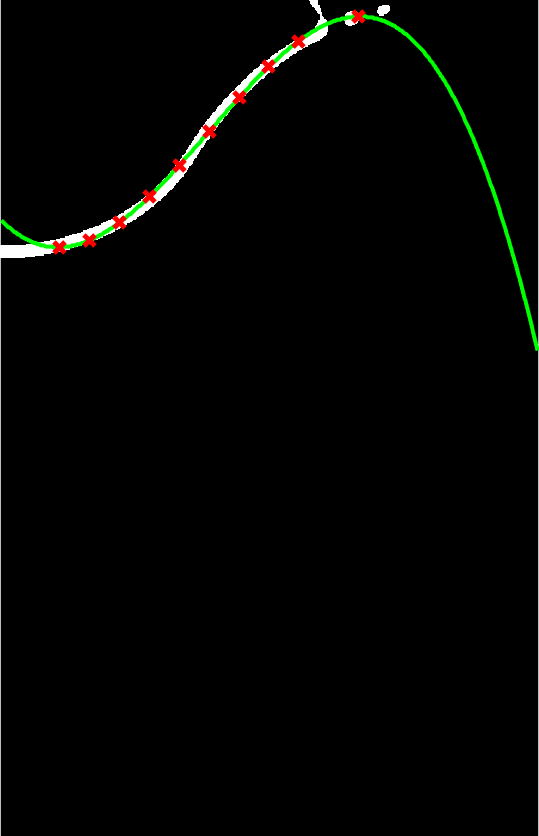
\includegraphics[width=0.3\textwidth]{fahrspurerkennung_ransac_imgRansacLeft.png}}
%  \quad
%  \subfloat[][]{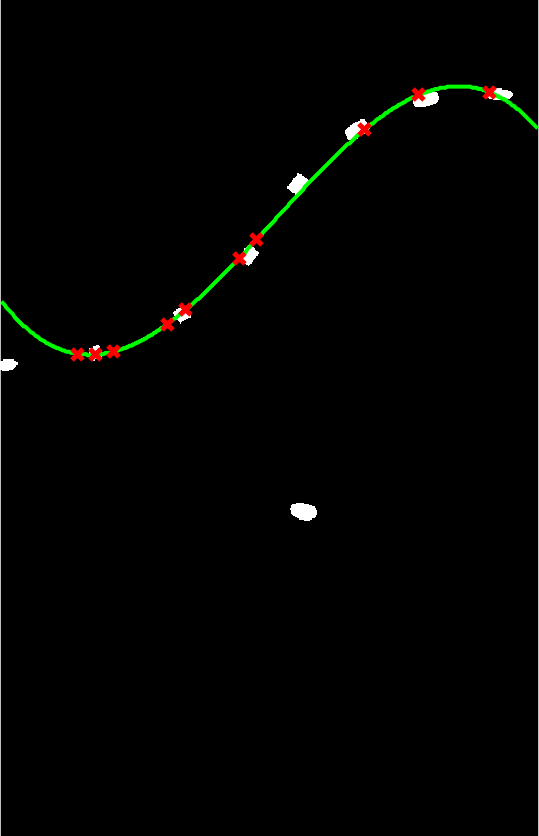
\includegraphics[width=0.3\textwidth]{fahrspurerkennung_ransac_imgRansacMiddle.png}}
%  \quad
%  \subfloat[][]{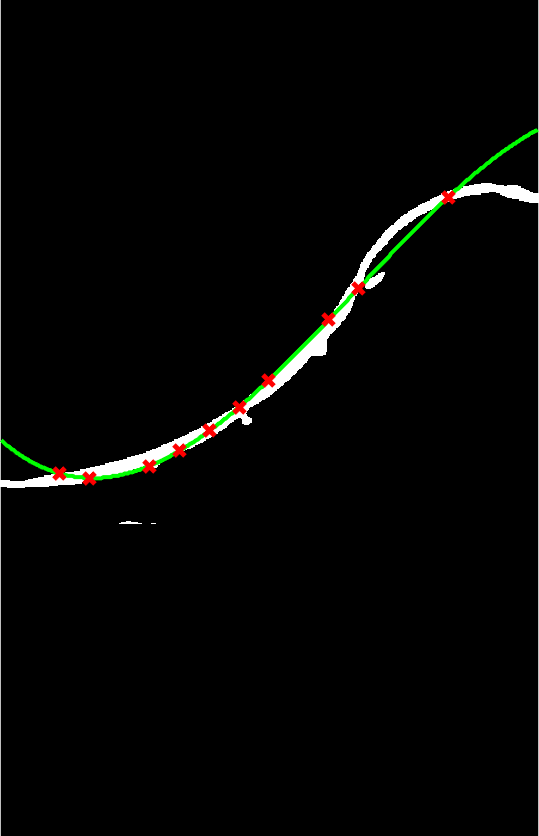
\includegraphics[width=0.3\textwidth]{fahrspurerkennung_ransac_imgRansacRight.png}}
%  \caption{Approximation der linken (a), mittleren (b) und rechten (c) Fahrbahnmarkierungen durch eine Funktion dritten Grades mittels \gls{acr:ransac}}
%\label{fig:fahrspurerkennung_ransac_ransac}
%\end{figure} 

\paragraph{\gls{acr:ransac} und Weltkarte} 
Wie in Abbildung~\ref{fig:fahrspurerkennung_ransac_masken} zu sehen, approximiert der \gls{acr:ransac}-Algorithmus den Verlauf der Fahrbahnlinien relativ gut. Die eingezeichnete grüne Funktion beschreibt das Ergebnis des Fits eines Polynoms dritten Grades durch die Inlier (siehe Abschnitt \ref{ssec:grunglagen:ransac:ablauf}). In einem bestimmten Abstand werden auf dem Polynom potentielle Kartenpunkte diskretisiert. Später tragen wir in die Karte nur die Punkte ein, welche sowohl auf der Funktion liegen als auch mit weißen Pixeln des maskierten Bildes übereinstimmen. So verhindern wir, Punkte an unpassenden Stellen in die Weltkarte einzutragen. 